\documentclass{standalone}
\usepackage{tikz}
\usetikzlibrary{patterns, positioning}
\usepackage[sfdefault]{ClearSans} %% option 'sfdefault' activates Clear Sans as the default text font
\usepackage[T1]{fontenc}

\begin{document}
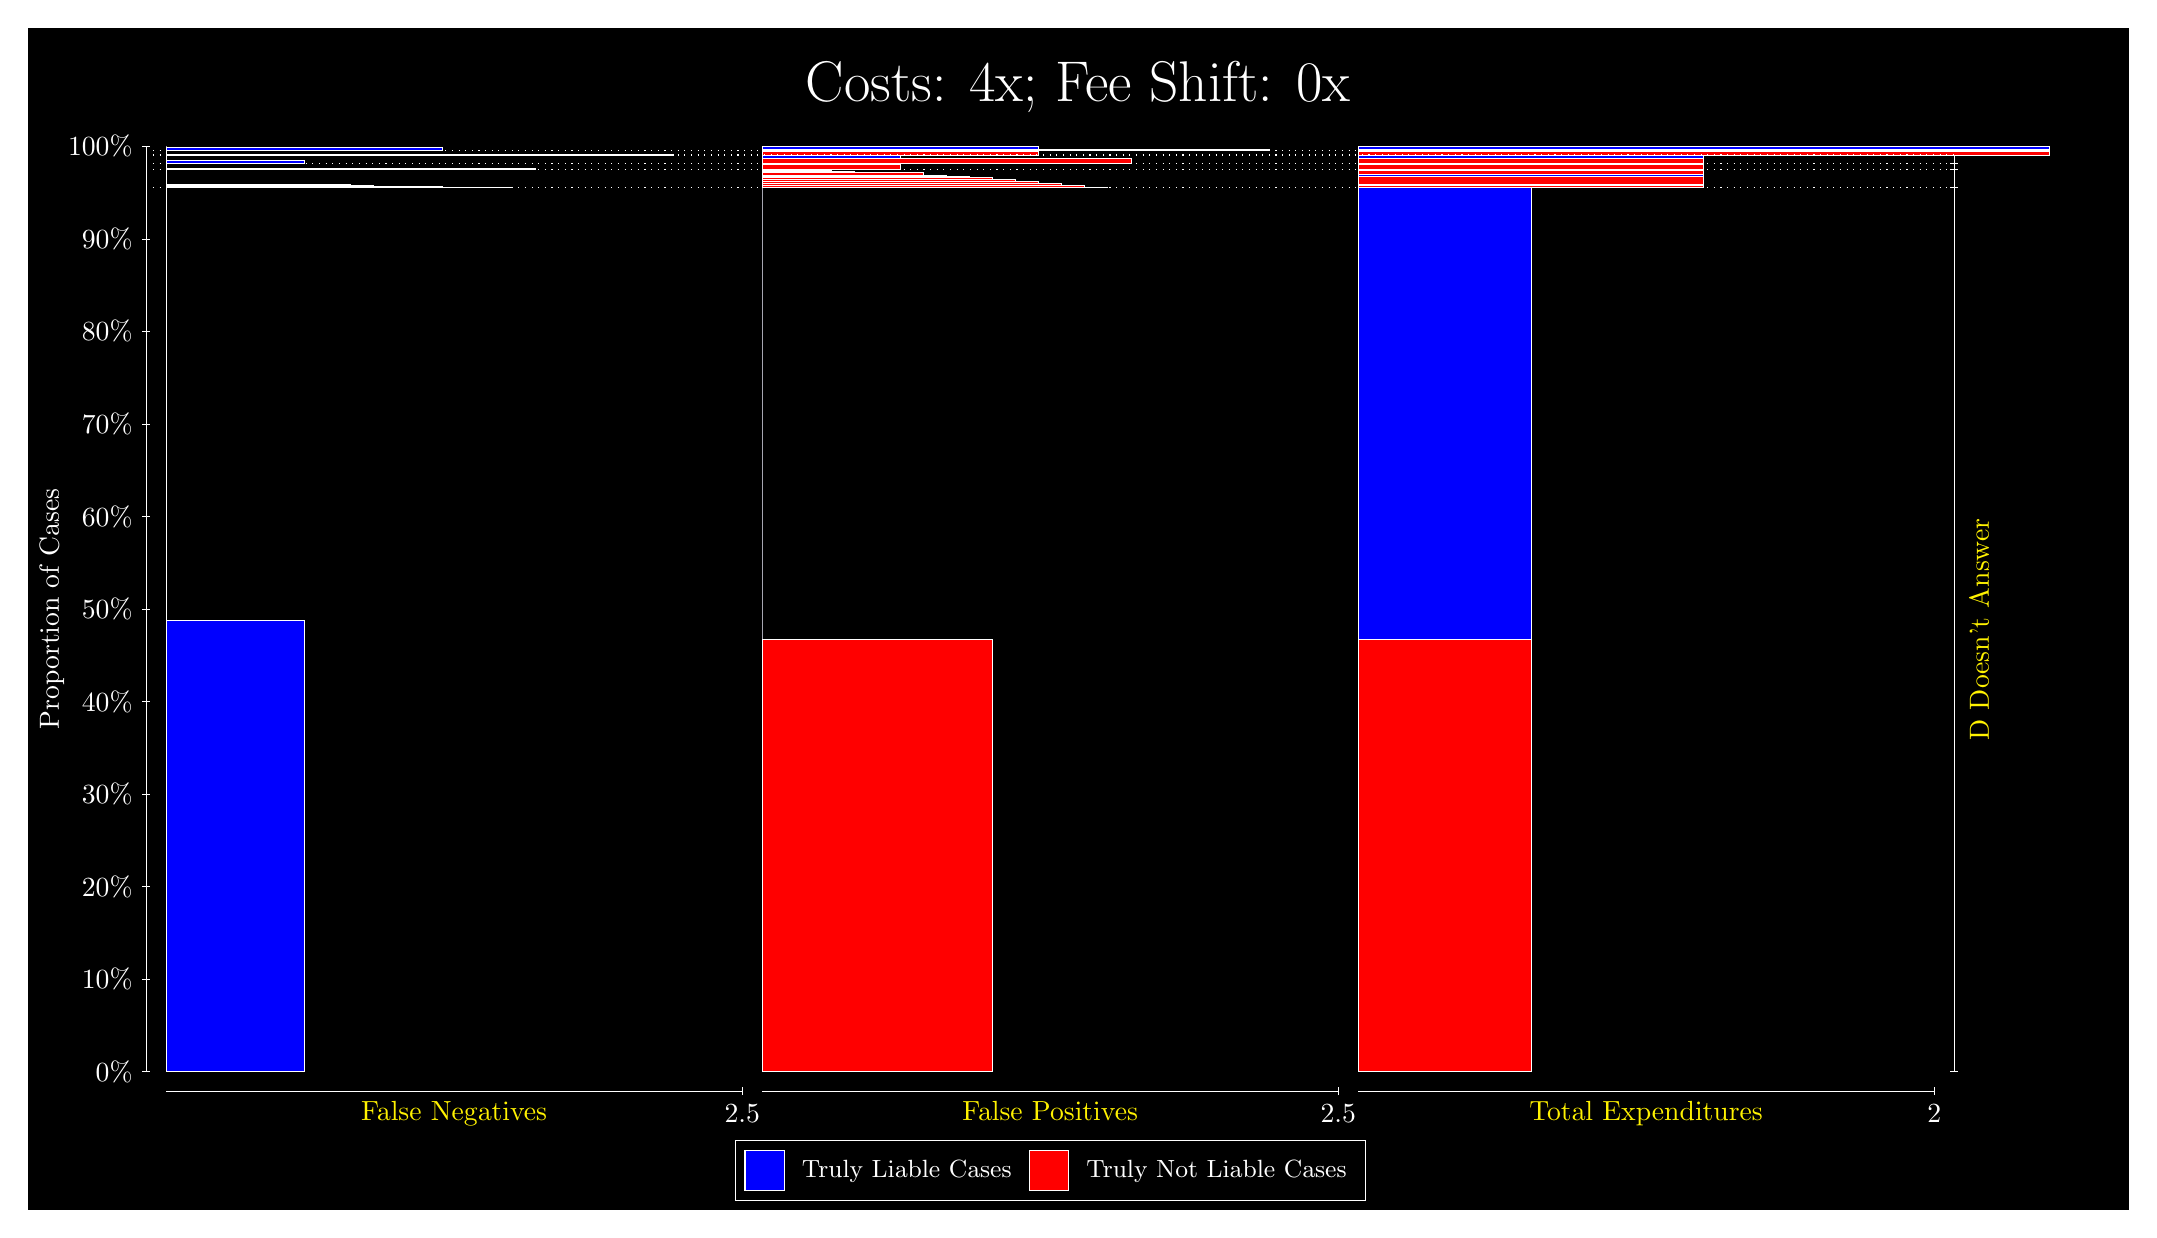
\begin{tikzpicture}
\draw[fill=black] (0,0) rectangle (26.667,15);
\draw[text=white] (0,13.5) rectangle (26.667,15) node[midway] {\huge Costs: 4x; Fee Shift: 0x};
\draw[white, very thin] (1.5,1.75) -- (1.5,13.5);
\node[rotate=90, text=white, anchor=center] at (0.3, 7.625) {Proportion of Cases};
\draw[white, very thin] (1.45,1.75) -- (1.55,1.75);
\node[text=white, anchor=east] at (1.45, 1.75) {0\%};
\draw[white, very thin] (1.45,2.925) -- (1.55,2.925);
\node[text=white, anchor=east] at (1.45, 2.925) {10\%};
\draw[white, very thin] (1.45,4.1) -- (1.55,4.1);
\node[text=white, anchor=east] at (1.45, 4.1) {20\%};
\draw[white, very thin] (1.45,5.275) -- (1.55,5.275);
\node[text=white, anchor=east] at (1.45, 5.275) {30\%};
\draw[white, very thin] (1.45,6.45) -- (1.55,6.45);
\node[text=white, anchor=east] at (1.45, 6.45) {40\%};
\draw[white, very thin] (1.45,7.625) -- (1.55,7.625);
\node[text=white, anchor=east] at (1.45, 7.625) {50\%};
\draw[white, very thin] (1.45,8.8) -- (1.55,8.8);
\node[text=white, anchor=east] at (1.45, 8.8) {60\%};
\draw[white, very thin] (1.45,9.975) -- (1.55,9.975);
\node[text=white, anchor=east] at (1.45, 9.975) {70\%};
\draw[white, very thin] (1.45,11.15) -- (1.55,11.15);
\node[text=white, anchor=east] at (1.45, 11.15) {80\%};
\draw[white, very thin] (1.45,12.325) -- (1.55,12.325);
\node[text=white, anchor=east] at (1.45, 12.325) {90\%};
\draw[white, very thin] (1.45,13.5) -- (1.55,13.5);
\node[text=white, anchor=east] at (1.45, 13.5) {100\%};

\draw[white, very thin] (24.457,1.75) -- (24.457,13.5);
\draw[white, very thin] (24.407,1.75) -- (24.507,1.75);
\node[anchor=west] at (24.407, 1.75) {};
\draw[white, very thin] (24.407,12.977) -- (24.507,12.977);
\node[anchor=west] at (24.407, 12.977) {};
\draw[white, very thin] (24.407,13.211) -- (24.507,13.211);
\node[anchor=west] at (24.407, 13.211) {};
\draw[white, very thin] (24.407,13.287) -- (24.507,13.287);
\node[anchor=west] at (24.407, 13.287) {};
\draw[white, very thin] (24.407,13.39) -- (24.507,13.39);
\node[anchor=west] at (24.407, 13.39) {};
\draw[white, very thin] (24.407,13.452) -- (24.507,13.452);
\node[anchor=west] at (24.407, 13.452) {};
\draw[white, very thin] (24.407,13.5) -- (24.507,13.5);
\node[anchor=west] at (24.407, 13.5) {};

\draw[white, very thin, fill=blue] (1.75,1.75) rectangle (3.5065,7.4815);
\draw[white, very thin, fill=red] (1.75,7.4815) rectangle (1.75,12.977);
\draw[white, very thin, fill=blue] (1.75,12.977) rectangle (6.1413,12.981);
\draw[white, very thin, fill=blue] (1.75,12.981) rectangle (5.8486,12.983);
\draw[white, very thin, fill=blue] (1.75,12.983) rectangle (5.5558,12.986);
\draw[white, very thin, fill=blue] (1.75,12.986) rectangle (5.2631,12.988);
\draw[white, very thin, fill=blue] (1.75,12.988) rectangle (4.9703,12.994);
\draw[white, very thin, fill=blue] (1.75,12.994) rectangle (4.6775,12.998);
\draw[white, very thin, fill=blue] (1.75,12.998) rectangle (4.3848,13.007);
\draw[white, very thin, fill=blue] (1.75,13.007) rectangle (4.092,13.015);
\draw[white, very thin, fill=blue] (1.75,13.015) rectangle (3.7993,13.024);
\draw[white, very thin, fill=red] (1.75,13.024) rectangle (1.75,13.211);
\draw[white, very thin, fill=blue] (1.75,13.211) rectangle (6.4341,13.221);
\draw[white, very thin, fill=red] (1.75,13.221) rectangle (1.75,13.287);
\draw[white, very thin, fill=blue] (1.75,13.287) rectangle (3.5065,13.326);
\draw[white, very thin, fill=red] (1.75,13.326) rectangle (1.75,13.39);
\draw[white, very thin, fill=blue] (1.75,13.39) rectangle (8.1906,13.401);
\draw[white, very thin, fill=red] (1.75,13.401) rectangle (1.75,13.452);
\draw[white, very thin, fill=blue] (1.75,13.452) rectangle (5.2631,13.49);
\draw[white, very thin, fill=red] (1.75,13.49) rectangle (1.75,13.5);
\draw[white, very thin, fill=red] (9.3189,1.75) rectangle (12.246,7.2455);
\draw[white, very thin, fill=blue] (9.3189,7.2455) rectangle (9.3189,12.977);
\draw[white, very thin, fill=red] (9.3189,12.977) rectangle (13.71,12.985);
\draw[white, very thin, fill=red] (9.3189,12.985) rectangle (13.417,13);
\draw[white, very thin, fill=red] (9.3189,13) rectangle (13.125,13.031);
\draw[white, very thin, fill=red] (9.3189,13.031) rectangle (12.832,13.054);
\draw[white, very thin, fill=red] (9.3189,13.054) rectangle (12.539,13.087);
\draw[white, very thin, fill=red] (9.3189,13.087) rectangle (12.246,13.105);
\draw[white, very thin, fill=red] (9.3189,13.105) rectangle (11.954,13.122);
\draw[white, very thin, fill=red] (9.3189,13.122) rectangle (11.661,13.134);
\draw[white, very thin, fill=red] (9.3189,13.134) rectangle (11.368,13.165);
\draw[white, very thin, fill=blue] (9.3189,13.165) rectangle (10.783,13.174);
\draw[white, very thin, fill=blue] (9.3189,13.174) rectangle (10.49,13.181);
\draw[white, very thin, fill=blue] (9.3189,13.181) rectangle (10.197,13.191);
\draw[white, very thin, fill=blue] (9.3189,13.191) rectangle (9.9044,13.194);
\draw[white, very thin, fill=blue] (9.3189,13.194) rectangle (9.6116,13.2);
\draw[white, very thin, fill=blue] (9.3189,13.2) rectangle (9.3189,13.211);
\draw[white, very thin, fill=red] (9.3189,13.211) rectangle (11.075,13.277);
\draw[white, very thin, fill=blue] (9.3189,13.277) rectangle (9.3189,13.287);
\draw[white, very thin, fill=red] (9.3189,13.287) rectangle (14.003,13.351);
\draw[white, very thin, fill=blue] (9.3189,13.351) rectangle (11.075,13.39);
\draw[white, very thin, fill=red] (9.3189,13.39) rectangle (12.832,13.441);
\draw[white, very thin, fill=blue] (9.3189,13.441) rectangle (9.9044,13.452);
\draw[white, very thin, fill=red] (9.3189,13.452) rectangle (15.759,13.462);
\draw[white, very thin, fill=blue] (9.3189,13.462) rectangle (12.832,13.5);
\draw[white, very thin, fill=red] (16.888,1.75) rectangle (19.083,7.2455);
\draw[white, very thin, fill=blue] (16.888,7.2455) rectangle (19.083,12.977);
\draw[white, very thin, fill=red] (16.888,12.977) rectangle (21.279,13.011);
\draw[white, very thin, fill=blue] (16.888,13.011) rectangle (21.279,13.016);
\draw[white, very thin, fill=red] (16.888,13.016) rectangle (21.279,13.124);
\draw[white, very thin, fill=blue] (16.888,13.124) rectangle (21.279,13.148);
\draw[white, very thin, fill=red] (16.888,13.148) rectangle (21.279,13.194);
\draw[white, very thin, fill=blue] (16.888,13.194) rectangle (21.279,13.211);
\draw[white, very thin, fill=red] (16.888,13.211) rectangle (21.279,13.277);
\draw[white, very thin, fill=blue] (16.888,13.277) rectangle (21.279,13.287);
\draw[white, very thin, fill=red] (16.888,13.287) rectangle (21.279,13.351);
\draw[white, very thin, fill=blue] (16.888,13.351) rectangle (21.279,13.39);
\draw[white, very thin, fill=red] (16.888,13.39) rectangle (25.67,13.441);
\draw[white, very thin, fill=blue] (16.888,13.441) rectangle (25.67,13.452);
\draw[white, very thin, fill=red] (16.888,13.452) rectangle (25.67,13.462);
\draw[white, very thin, fill=blue] (16.888,13.462) rectangle (25.67,13.5);
\draw[white, dotted] (1.5,12.977) -- (24.457,12.977);
\draw[white, dotted] (1.5,13.211) -- (24.457,13.211);
\draw[white, dotted] (1.5,13.287) -- (24.457,13.287);
\draw[white, dotted] (1.5,13.39) -- (24.457,13.39);
\draw[white, dotted] (1.5,13.452) -- (24.457,13.452);
\draw[white, very thin] (1.75,1.5) -- (9.0689,1.5);
\node[text=yellow, anchor=north] at (5.4094, 1.5) {False Negatives};
\draw[white, very thin] (9.0689,1.45) -- (9.0689,1.55);
\node[text=white, anchor=north] at (9.0689, 1.45) {2.5};

\draw[white, very thin] (9.3189,1.5) -- (16.638,1.5);
\node[text=yellow, anchor=north] at (12.978, 1.5) {False Positives};
\draw[white, very thin] (16.638,1.45) -- (16.638,1.55);
\node[text=white, anchor=north] at (16.638, 1.45) {2.5};

\draw[white, very thin] (16.888,1.5) -- (24.207,1.5);
\node[text=yellow, anchor=north] at (20.547, 1.5) {Total Expenditures};
\draw[white, very thin] (24.207,1.45) -- (24.207,1.55);
\node[text=white, anchor=north] at (24.207, 1.45) {2};

\node[text=yellow, centered, rotate=90] at (24.777, 7.3635) {D Doesn't Answer};






\draw (12.978300999999998,1.5) node[draw=none] (baseCoordinate) {};
\begin{scope}[align=center]
        \matrix[scale=0.5, draw=white, below=0.5cm of baseCoordinate, nodes={draw}, column sep=0.1cm]{
            \node[rectangle, draw, minimum width=0.5cm, minimum height=0.5cm, fill=blue] {}; &
            \node[draw=none, font=\small, text=white] (B) {Truly Liable Cases}; &
            \node[rectangle, draw, minimum width=0.5cm, minimum height=0.5cm, fill=red] {}; &
            \node[draw=none, font=\small, text=white] (B) {Truly Not Liable Cases}; \\
            };
\end{scope}

\end{tikzpicture}
\end{document}